\documentclass{article}
\usepackage{multicol}
\usepackage[english]{babel}
\usepackage{cite}
\usepackage{setspace}
\usepackage{amsmath}
\usepackage{nameref}
\usepackage[round]{natbib}
\usepackage{hyperref}
\usepackage{graphicx}
\usepackage{caption}
\usepackage{subcaption}
\usepackage{amsthm}
\usepackage[utf8]{inputenc}

\usepackage{tikz}
\usetikzlibrary{arrows}

\usepackage{amsthm}
\usepackage{cleveref}

% Page length commands go here in the preamble
\setlength{\oddsidemargin}{-0.25in} % Left margin of 1 in + 0 in = 1 in
\setlength{\textwidth}{7in}   % Right margin of 8.5 in - 1 in - 6.5 in = 1 in
\setlength{\topmargin}{-.75in} % Top margin of 2 in -0.75 in = 1 in
\setlength{\textheight}{9.2in}  % Lower margin of 11 in - 9 in - 1 in = 1 in


\theoremstyle{definition}
\newtheorem{mydef}{Definition}

\usepackage[T1]{fontenc}
\usepackage[utf8]{inputenc}
\usepackage{authblk}

\title{dr-disco intronic}

\author[1]{Youri Hoogstrate}
\affil[1]{Department of Urology, Erasmus University Medical Center}




\begin{document}
\maketitle

%\singlespacing
%	\begin{abstract}\textbf{}
%	\end{abstract}

%	\begin{center}
%	\line(1,0){250}
%	\end{center}
%\newpage
%\tableofcontents
%\newpage

\twocolumn
%\doublespace

\section{Methods}
The tool \textit{dr-disco intronic} tool tries to estimate break points on 2 levels: the exon-exon and the intron-intron boundaries (in case of an intron to intron DNA break point). It takes several steps to accomplish this, described below:

\clearpage

\subsection{Data structure}
The input for \textit{dr-disco} is an alignment file in the BAM format, that specifically contains discordant reads produced by RNA-STAR.
Typically those alignments contain aligned reads with an insert sizes that are either too small (e.g. overlapping the other mate) or too large (exceeding any reasonable exon length).
The former may be evidence for small local indels or inversions, but seem to occur most often due to library preparation. Therefore we deliberately filter those out.
For this we use the criterion that the distance between the aligned reads must at least be larger than the insert size. Because the insert size is $~sim 300bp$ and we want to have a certain confidence, also for other functions, we set the insert size to $1.5 \times$ insert size$=450bp$). Hence, we filter out discordant reads if they are smaller than this size and aligned to the same chromosome.
% Todo: give absolute stats on percentage removal
Remaining reads can either be classified into \textit{singletons} or \textit{paired end reads}.
Singletons are reads of which one of the mates was excluded from the alignment while the alignment of the remaining mate was considered discordant.
With BAM/SAM specification it is not possible to describe an inter-chromosomal junction into one single entry.
In RNA-STARs discordant alignment files discordant reads are being split up into two separate alignments, i.e. two entries, of which one is classified as \textit{secondary alignment}.
Hence, discordant reads are represented with doubles or triples of aligned reads for singletons and paired end reads.

The main data structure of this application is a \textit{graph}. There are typically two types of split reads; all singletons are considered to be split reads while paired end reads are only considered split reads if one of the mates is split up.
The remaining mate is then considered a \textit{silent mate} because it only anchors the alignment.
Spanning reads are a double of paired end reads of which none has been split up.
We classify such reads as follows:
\begin{itemize}
	\item Split read
	\begin{itemize}
		\item Singleton aligned chunk 1 \& singleton aligned chunk 2
		\item PE-R1 aligned chunk 1 \& PE-R1 aligned chunk 2 \& silent mate R2
		\item PE-R2 aligned chunk 1 \& PE-R2 aligned chunk 2 \& silent mate R1
	\end{itemize}
	\item Spanning read (double of discordant mates only)
	\begin{itemize}
		\item Paired end R1 read \& Paired end R2 read
	\end{itemize}
	\item Silent mate (triple of discordant mates only)
	\begin{itemize}
		\item PE-R1 aligned chunk 1 \& PE-R1 aligned chunk 2 \& silent mate R2
		\item PE-R2 aligned chunk 1 \& PE-R2 aligned chunk 2 \& silent mate R1
	\end{itemize}
\end{itemize}

According to the subtype and additional information (e.g. strand and clipping flags) the breakpoints and strands of the junction are estimated.
Also, if an aligned chunk contains a splice junction or and indel annotation, this will be considered as a separate type of junction and will be included in the graph as well.
If any of the two breakpoints of a junction does not exist, the position will be inserted into the graph as a \textit{node}.
When all nodes of a junction are present in the graph, and the edge between the two positions does not exists in the graph, the junction will be inserted as a (bi-directional) \textit{edge} into the graph, connecting the two corresponding breakpoints.
The edge will be annotated such that the weight of the subtype of corresponding reads gets increased by one.
The nodes of the graph are also inserted into a genomic-range index (intervaltree-bio python package) to quickly target specific subregions in the graph.
Lastly, each node has a property describing the number of (soft/hard)-clips found in corresponding mates, illustrated in figure \ref{fig:edges_clips}.

\begin{figure}
% xref: http://tex.stackexchange.com/questions/45734/drawing-graphs-in-latex
\begin{tikzpicture}[->,>=stealth',shorten >=1pt,auto,node distance=3cm,
                    thick,main node/.style={circle,draw,font=\sffamily\Large\bfseries}]

  \node[main node] (1) {\small{chr1:100}};
  \node[main node] (2) [right of=1] {\small{chr2:900}};

  \path[every node/.style={font=\sffamily\small}]
    (1) edge [bend left] node {split: 1} (2)
        edge [loop below,color=gray] node {clips: 1} (1)
    (2) edge [bend left] node {split: 1} (1)
        edge [loop below,color=gray] node {clips: 0} (2)
;
\end{tikzpicture}
\caption{Left: graph before pruning, right: after pruning}
\label{fig:edges_clips}
\end{figure}

\clearpage


\subsection{Pruning (the graph)}
Consider the alignment below as example we would like to transform into a graph:
\begin{verbatim}
chr1:
  80        90        100
..|....i....|....i....|....i..
      [----read-01----|
          [--read-02--|
[--read-03--]


chr2:      
       900       910
..i....|....i....|....i....|..
       |--read-01--]
       |----read-02---]
                 [--read-03--]
\end{verbatim}
The corresponding graph would look like presented in figure \ref{fig:pruning_graph} (left).

\begin{figure*}
% xref: http://tex.stackexchange.com/questions/45734/drawing-graphs-in-latex
\begin{tikzpicture}[->,>=stealth',shorten >=1pt,auto,node distance=3cm,
                    thick,main node/.style={circle,draw,font=\sffamily\Large\bfseries}]

  \node[main node] (1) {\small{chr1:90}};
  \node[main node] (2) [right of=1] {\small{chr1:100}};
  \node[main node] (3) [right of=2] {\small{chr2:900}};
  \node[main node] (4) [right of=3] {\small{chr2:910}};

  \path[every node/.style={font=\sffamily\small}]
    (1) edge [bend left] node {discordant: 1} (4)
%        edge [loop below] node {clips: 0} (4)
    (2) edge [bend left] node {split: 2} (3)
%        edge [loop below] node {clips: 0} (3)
    (3) edge [bend left] node {split: 2} (2)
%        edge [loop below] node {clips: 0} (2)
    (4) edge [bend left] node {discordant: 1} (1)
%        edge [loop below] node {clips: 0} (1)
;
\end{tikzpicture}
\begin{tikzpicture}[->,>=stealth',shorten >=1pt,auto,node distance=3cm,
                    thick,main node/.style={circle,draw,font=\sffamily\Large\bfseries}]

  \node[main node] (1) {\small{chr1:100}};
  \node[main node] (2) [right of=2] {\small{chr2:900}};

  \path[every node/.style={font=\sffamily\small}]
    (1) edge [bend left] node [text width=2cm,align=center]{split: 2, \\ discordant$^*$: 1} (2)
    (2) edge [bend left] node [text width=2cm,align=center]{split: 2, \\ discordant$^*$: 1} (1)
;
\end{tikzpicture}
\caption{Left: graph before pruning, right: after pruning}
\label{fig:pruning_graph}
\end{figure*}

Hence, in this graph each node is a genomic location and edges represent the junctions in the alignment.
The graph contains two split reads that break from \verb|chr1:100| to \verb|chr2:900| and a spanning read aligned from \verb|chr1:90| to \verb|chr2:910|.
In this graph we have actually very closely adjacent edges; the edges with split and discordant reads differ on both nodes not more than 10bp.
It is very likely that those two edges are actually coming from the same genomic event.
Discordant reads do usually not cover the actual break point but are closely adjacent while on the other hand split reads should be falling on the break exactly.
In order to combine this information, this distance of each of the nodes needs to be reasonable, which would mean for the sequencing data that it should not exceed the insert size of the sequencing reads.
Therefore we added the pruning step that merges edges of this type together.

Pruning starts by finding the edge with the highest weight, looking for both its corresponding vertices for arcs that have their edges in no more than the insert size (450bp) away and are in the same orientation.
Because split reads have a higher probability to be exactly on the break point, they have an increased weight for estimating the highest weight.

The data structure of the pruned example is given in figure \ref{fig:pruning_graph} (right).
Although the total weight of all edges stays identical, the number of edges and nodes shall decrease with every pruning operation and the graph shall become smaller in size.
Splice junctions are not taken into account in the pruning function.

\clearpage

\subsection{Re-joining splice junctions}
% What does this function do:
% - Add splice junctions to all nodes?
% - Link nodes to each othed based on splice junctions? (I suppose it does both, which makes it easy to pull them down)
%
%if left_junc[1] != None:
%    node1.splice_edges[node2] = left_junc
%    node2.splice_edges[node1] = left_junc

Each splice junction is represented as an edge between two nodes.
However, different non-splice junctions may correspond to the same genomic event, due to alternative splicing.
Currently, a breakpoint of a junction on the opposite side or in the middle of an exon it is not directly connected to the splice junction although it is in close proximity.
Therefore it is desired to have the exon junctions connected to all junctions in close proximity.
In other words, it would be desired to have the junctions themselves being directly connected to each other by the splice junctions.
This step is referred to as \textit{re-joining splice junction(s)}.
We would like to include the splice junctions to \textbf{all} edges that are in close proximity (450bp), possibly resulting into one splice junction linking several nodes together.

\begin{verbatim}
edges (junctions):
          -------- ... ------        j1
     ------------- ... ------        j2
     ------------- ... ------------- j3
------------------ ... ------------- j4
nodes (genomic positions):
|   |    |                   |     |

 splice juncs:
 --- ----                     -----
:   :    :        ...        :     :
\end{verbatim}
In the example above we have 4 junctions ($j_1,\ldots,j_4$).

Instead of adding the splice junctions to the Graph, we re-insert them as properties of the Nodes.

%% Has to be changes / improved
The prodedure goes as follows:
...
For every `thicker\_edge', hence, edge returned after pruning, 


\begin{figure*}
% xref: http://tex.stackexchange.com/questions/45734/drawing-graphs-in-latex
\begin{tikzpicture}[->,>=stealth',shorten >=1pt,auto,node distance=3cm,
                    thick,main node/.style={circle,draw,font=\sffamily\Large\bfseries}]

  \node[main node] (1) {\small{chr1:1000}};
  \node[main node] (2) [right of=1,color=gray] {\small{chr1:1250}};
  \node[main node] (3) [right of=2,color=gray] {\small{chr1:2400}};
  \node[main node] (4) [right of=3] {\small{chr1:2500}};
  \node[main node] (5) [right of=4] {\small{chr2:200}};

  \path[every node/.style={font=\sffamily\small}]
    (1) edge [bend left] node {discordant: 1} (5)
    (2) edge [bend left,color=gray] node {splice: 1} (3)
    (3) edge [bend left,color=gray] node {splice: 1} (2)
    (4) edge [bend left] node {split: 2} (5)
    (5) edge [bend left] node {split: 2} (4)
    (5) edge [bend left] node {discordant: 1} (1)
;
\end{tikzpicture}

\begin{tikzpicture}[->,>=stealth',shorten >=1pt,auto,node distance=3cm,
                    thick,main node/.style={circle,draw,font=\sffamily\Large\bfseries}]

  \node[main node] (1) {\small{chr1:1000}};
  \node[main node] (2) [right of=1,color=gray] {\small{chr1:1250}};
  \node[main node] (3) [right of=2,color=gray] {\small{chr1:2400}};
  \node[main node] (4) [right of=3] {\small{chr1:2500}};
  \node[main node] (5) [right of=4] {\small{chr2:200}};

  \path[every node/.style={font=\sffamily\small}]
    (1) edge [bend left] node {discordant: 1} (5)
    (2) edge [bend left,color=gray] node {splice: 1} (3)
    (3) edge [bend left,color=gray] node {splice: 1} (2)

    (1) edge [color=gray,dotted] node {s-link} (2)
    (2) edge [color=gray,dotted] node {$d_1=250$} (1)
    (3) edge [color=gray,dotted] node {s-link} (4)
    (4) edge [color=gray,dotted] node {$d_2=100$} (3)
    
    (4) edge [bend left] node {split: 2} (5)
    (5) edge [bend left] node {split: 2} (4)
    (5) edge [bend left] node {discordant: 1} (1)
;
\end{tikzpicture}

\caption{Merge SJ}
\label{fig:merge_sj}
\end{figure*}

\clearpage

\subsection{Extract subnetworks}
In the previous step nodes have been connected by all splice junctions in close proximity.
Therefore it is possible to extract corresponding junctions as a network, by recursively traversing their splice junctions.
To ensure we may not miss any in-between edges, we will pull down all nodes first, and look for all existing edges in-between.
We start with the highest scoring edge (2 split reads):


\begin{tikzpicture}[->,>=stealth',shorten >=1pt,auto,node distance=3cm,
                    thick,main node/.style={circle,draw,font=\sffamily\Large\bfseries}]

  \node[main node] (4) [right of=3] {\small{chr1:2500}};
  \node[main node] (5) [right of=4] {\small{chr2:200}};

  \path[every node/.style={font=\sffamily\small}]
    (4) edge [bend left] node {split: 2} (5)
    (5) edge [bend left] node {split: 2} (4)
;
\end{tikzpicture}

\noindent We then take the breakpoints apart, and for each of them recursively find nodes connected by splice junctions.
Key in this problem is that every junction may not be further away (in transcript length) than the insert size.
Therefore we can do this recursively, with a recursion constraint based on the travelled exonic distance.


In the following example we have two junctions ($j_1$ and $j_2$) that are in adjacent exons.
In our data structure there are no exons, just splice junctions (SJ).
In the following example we see how the data looks like:
\begin{verbatim}
            ___sj____
           |         |
---[ exon1 ]---------[ exon2 ]--
aatagcatcgatcgacttagctacgaacacag
      |                |______ j1 ___
      |_______________________ j2 ___
\end{verbatim}
While in the data structure this looks more like this:
\begin{verbatim}
            ___sj____
           |         |
-------------------------------------
      |                |______ j1 ___
      |_______________________ j2 ___
\end{verbatim}
We start extracting the subnetwork by the junction with the highest score, i.e. number of corresponding reads.
Let's  assume the start point is $j_1$, and the chosen insert size if 15.
We need to find all splice junctions that are in less than the insert size available (\verb|=|):
\begin{verbatim}
            ___sj____
           |         |
---------------------===-------------
      |                |______ j1 ___
      |_______________________ j2 ___
\end{verbatim}
For that splice junction, the distance to the next junction may not be longer than $15-3=12$.
Fortunately, if we travel from the other end of \textit{SJ} to the end of $j_2$, we travel only 6 more bases (\verb|:|):
\begin{verbatim}
            ___sj____
           |         |
------::::::---------===-------------
      |                |______ j1 ___
      |_______________________ j2 ___
\end{verbatim}



\subsection{Merge overlapping subnets}
It may be possible that novel or unannotated exons exist and certain junctions did not get connected to the subnetwork by splice junctions.
A typical example is exon-0 in the TMPRSS2-ERG fusion gene.
To also include those junctions, we merge subnetworks together based on their overall distance to other networks.
This is because it often happens that novel exons are being used or that no splice junctions were present in the alignment.
This may also merge intronic with splice-junction spanning reads.
We apply a filter on the subnetworks that uses the number of discordant reads, split reads and entropy (unique aligned reads in contrast to all reads involved).

The reads spanning the genomic break point are most often not connected by any other read to the reads spanning the nearest splice junctions.
They both end up in a separate 'network' of reads, to be merged afterwards:

Merges very closely adjacent subnets based on the smallest internal distance.
E.g. if we have a subnet having 1 and one having 2 edges:

\begin{verbatim}
  snA:  |       |            ~             |
        |        --------------------------  edgeA1
         ----------------------------------  edgeA2

  snB         |                        |
               ------------------------      edgeB1


\end{verbatim}        

        We would like to filter based on the distance between edgeA1 and
        edgeB1.
        
        We also don't want to have a growth pattern, i.e. that based on
        merging snB to snA, snC becomes part of it. Although it may be
        true it can become problematc as I've seen with FuMa.
        
        So, idea is:
        loop over all subnets i;
            loop over all subnets j > i
                if subnet j should be merged with i, remeber it into M
            
            merge all subnets in M into i, and remove the former subnets


\end{document}

